%% V1.0
%% by Gabriel Garcia, gabrcg@gmail.com
%% This is a template for Udacity projects using IEEEtran.cls

%% Be Udacious!

\documentclass[10pt,journal,compsoc]{IEEEtran}

\usepackage[pdftex]{graphicx}    
\usepackage{cite}
\hyphenation{op-tical net-works semi-conduc-tor}
\usepackage{listings}
\usepackage{color}

\definecolor{dkgreen}{rgb}{0,0.6,0}
\definecolor{gray}{rgb}{0.5,0.5,0.5}
\definecolor{mauve}{rgb}{0.58,0,0.82}

\lstset{frame=tb,
  language=C++,
  aboveskip=3mm,
  belowskip=3mm,
  showstringspaces=false,
  columns=flexible,
  basicstyle={\small\ttfamily},
  numbers=none,
  numberstyle=\tiny\color{gray},
  keywordstyle=\color{blue},
  commentstyle=\color{dkgreen},
  stringstyle=\color{mauve},
  breaklines=true,
  breakatwhitespace=true,
  tabsize=3
}

\begin{document}

\title{Deep RL Arm Manipulation}

\author{Hsin-Wen Chang}

\markboth{Deep Reinforcement Learning Arm Manipulation, DQN, Robotics Software Engineer Nanodegree Program, Udacity}%
{}
\IEEEtitleabstractindextext{%

\begin{abstract}
The goal of this project is to create a DQN agent and define reward functions to teach a robotic arm to perform two primary objectives. one is aim to have any part of the robot arm touch the object of interest with at least a 90 percent accuracy. Second is aim for only the gripper base of the robot arm touch the object, with at least a 80 percent accuracy.
\end{abstract}

% Note that keywords are not normally used for peerreview papers.
\begin{IEEEkeywords}
Deep Reinforcement Learning Arm Manipulation, DQN, Robotics Software Engineer Nanodegree Program, Robot, IEEEtran, Udacity, \LaTeX.
\end{IEEEkeywords}}

\maketitle
\IEEEdisplaynontitleabstractindextext
\IEEEpeerreviewmaketitle
\section{Introduction}
\label{sec:introduction}

\IEEEPARstart{D}{ee}p Reinforcement Learning

\section{Background}
  %example for inserting image
\begin{figure}[thpb]
      \centering
      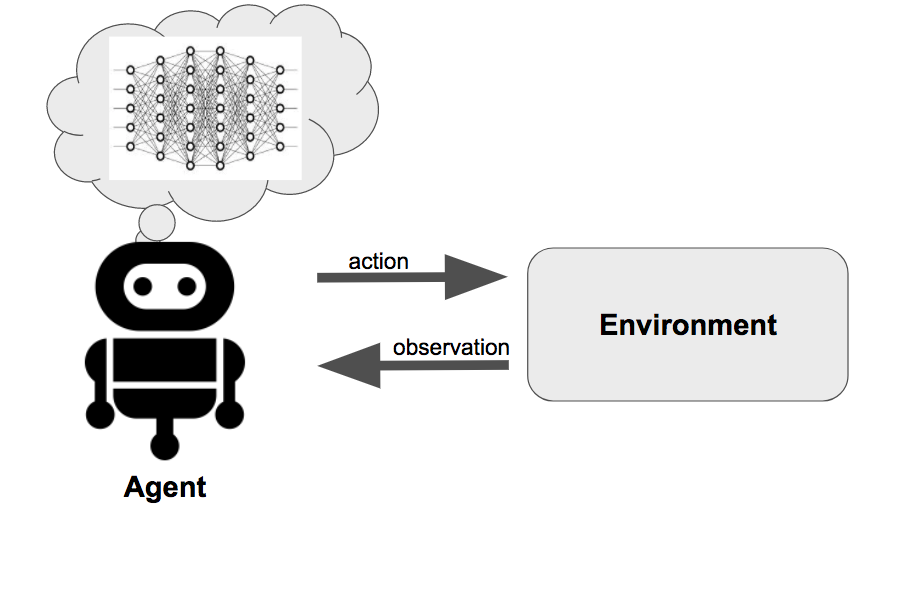
\includegraphics[width=\linewidth]{FromRLToDeepRL.png}
      \caption{From RL to Deep RL.}
      \label{fig:robot1}
\end{figure}
The difference between RL and Deep RL is the use of a deep neural network. Think of the collection of value-action pairs that define what actions an agent should take in any situation as a function of the observations that the agent receives from its environment. Neural network can be used to approximate this function because through its large quantity of parameters that can be learned through trial and error.
\subsection{Setup and building from Source (Nvidia Jetson TX2)}

\begin{lstlisting}
$ sudo apt-get install cmake
$ conda install -c pytorch pytorch
$ sudo apt-get install libignition-math2-dev
$ git clone http://github.com/udacity/RoboND-DeepRL-Project
$ cd RoboND-DeepRL-Project
$ git submodule update --init
$ mkdir build
$ cd build
$ cmake ../
$ make
\end{lstlisting}
%example for Bullet point list
\begin{itemize}
\item  Subscribe to camera topics:
\begin{lstlisting}
//Subscribe to camera topic
cameraSub = cameraNode->Subscribe("/gazebo/arm_world
/camera/link/camera/image", &ArmPlugin::onCameraMsg, this);
\end{lstlisting}
\item Subscribe to collision topics:
\begin{lstlisting}
// Subscribe to prop collision topic
collisionSub = collisionNode->Subscribe("/gazebo
/arm_world/tube/tube_link/my_contact", &ArmPlugin::onCollisionMsg, this);
\end{lstlisting}
\item Create the DQN Agent:
\begin{lstlisting}
// Create DQN Agent
agent = dqnAgent::Create(INPUT_WIDTH, INPUT_HEIGHT, INPUT_CHANNELS, NUM_ACTIONS, OPTIMIZER, LEARNING_RATE, REPLAY_MEMORY, BATCH_SIZE, GAMMA, EPS_START, EPS_END, EPS_DECAY,USE_LSTM, LSTM_SIZE, ALLOW_RANDOM, DEBUG_DQN);
\end{lstlisting}
\item Velocity or position based control of arm joints:

The DQN output is mapped to a particular action such as the control of each joint for the robotic arm. In ArmPlugin::updateAgent(), there are two existing approaches to control the joint movements.
\begin{lstlisting}
const int jointIndex = action / 2;
const int actionDirection = 1 - 2 * (action % 2);
//Increase or decrease the joint velocity based on whether the action is even or odd. Set joint velocity based on whether action is even or odd.
const float velocity = vel[jointIndex] + actionVelDelta * actionDirection; 
// Increase or decrease the joint position based on whether the action is even or odd Set joint position based on whether action is even or odd.
float joint = ref[jointIndex] + actionJointDelta * actionDirection;
\end{lstlisting}

\item Reward for robot gripper hitting the ground:
\begin{lstlisting}
// Get the bounding box for the gripper		
const math::Box& gripBBox = gripper->GetBoundingBox();
const float groundContact = 0.05f;
// Set appropriate Reward for robot hitting the ground.
const bool checkGroundContact =  ( gripBBox.min.z <= groundContact || gripBBox.max.z <= groundContact );
\end{lstlisting}
\end {itemize}

\subsection{Reward function design}

\begin{lstlisting}
const float distDelta  = lastGoalDistance - distGoal;
// Compute the smoothed moving average of the delta of the distance to the goal
avgGoalDelta  = (avgGoalDelta * ALPHA) + (distDelta * (1.0f - ALPHA));
\end{lstlisting}

%example for Bullet point list
\begin{itemize}
\item REWARD LOSS: When robotic arm can't completed it's a round task, this penalty will be issued.
\item REWARD WIN: When robotic arm completed its round task, this reward will be issued.
\item REWARD MUL: Base on the distance between the arm and the object use this distance to calculate an appropriate reward.
\end {itemize}

\subsection{DQN agent's hyperparameters}
\begin{itemize}
\item Initial Parameters:
\begin{lstlisting}
#define INPUT_WIDTH   512
#define INPUT_HEIGHT  512
#define OPTIMIZER "None"
#define LEARNING_RATE 0.0f
#define REPLAY_MEMORY 10000
#define BATCH_SIZE 8
#define USE_LSTM false
#define LSTM_SIZE 32

\end{lstlisting}
\item Parameters Tuned:

Input image size is quite large and influence memory usage. Reduce image size will improve performance. Optimizer were changed to RMSprop which is commonly used and produce good result.Small number learning rate will slow learning speed but minimize error. Smaller batch size will reduce more computing power.
\begin{lstlisting}
#define INPUT_WIDTH   64 
#define INPUT_HEIGHT  64
#define OPTIMIZER "RMSprop" 
#define LEARNING_RATE 0.9f 
#define REPLAY_MEMORY 10000
#define BATCH_SIZE 128  
#define USE_LSTM true
#define LSTM_SIZE 256

\end{lstlisting}
\end {itemize}
\begin{table}[h]
 \begin{center}
      \begin{tabular}{ |c|c| } 
       \hline
       Hyperparameters & Values \\
       \hline
       INPUT WIDTH & 64 \\ 
       INPUT HEIGHT & 64 \\
       INPUT CHANNELS & 3\\
       NUM ACTIONS & DOF*2 \\
       OPTIMIZER & RMSprop \\
       LEARNING RATE & 0.9f\\
       REPLAY MEMORY & 10000 \\
       BATCH SIZE & 128\\
       GAMMA & 0.9f\\
       EPS START & 0.9f\\
       EPS END & 0.0f \\
       EPS DECAY & 250\\
       USE LSTM & true\\
       LSTM SIZE & 256\\
       ALLOW RANDOM & true\\
       DEBUG DQN & false \\
       \hline
      \end{tabular}
      \caption{Table of hyperparameters}
      \label{table:1}
      \end{center}
      \end{table}
\section{Results}
Both task have trained with the parameters in TABLE 1 and the two primary objectives were achieved:
\begin{itemize}
\item Have any part of the robot arm touch the object of interest, with at least a 90 percent accuracy. 
\begin{figure}[htpb]
      \centering
      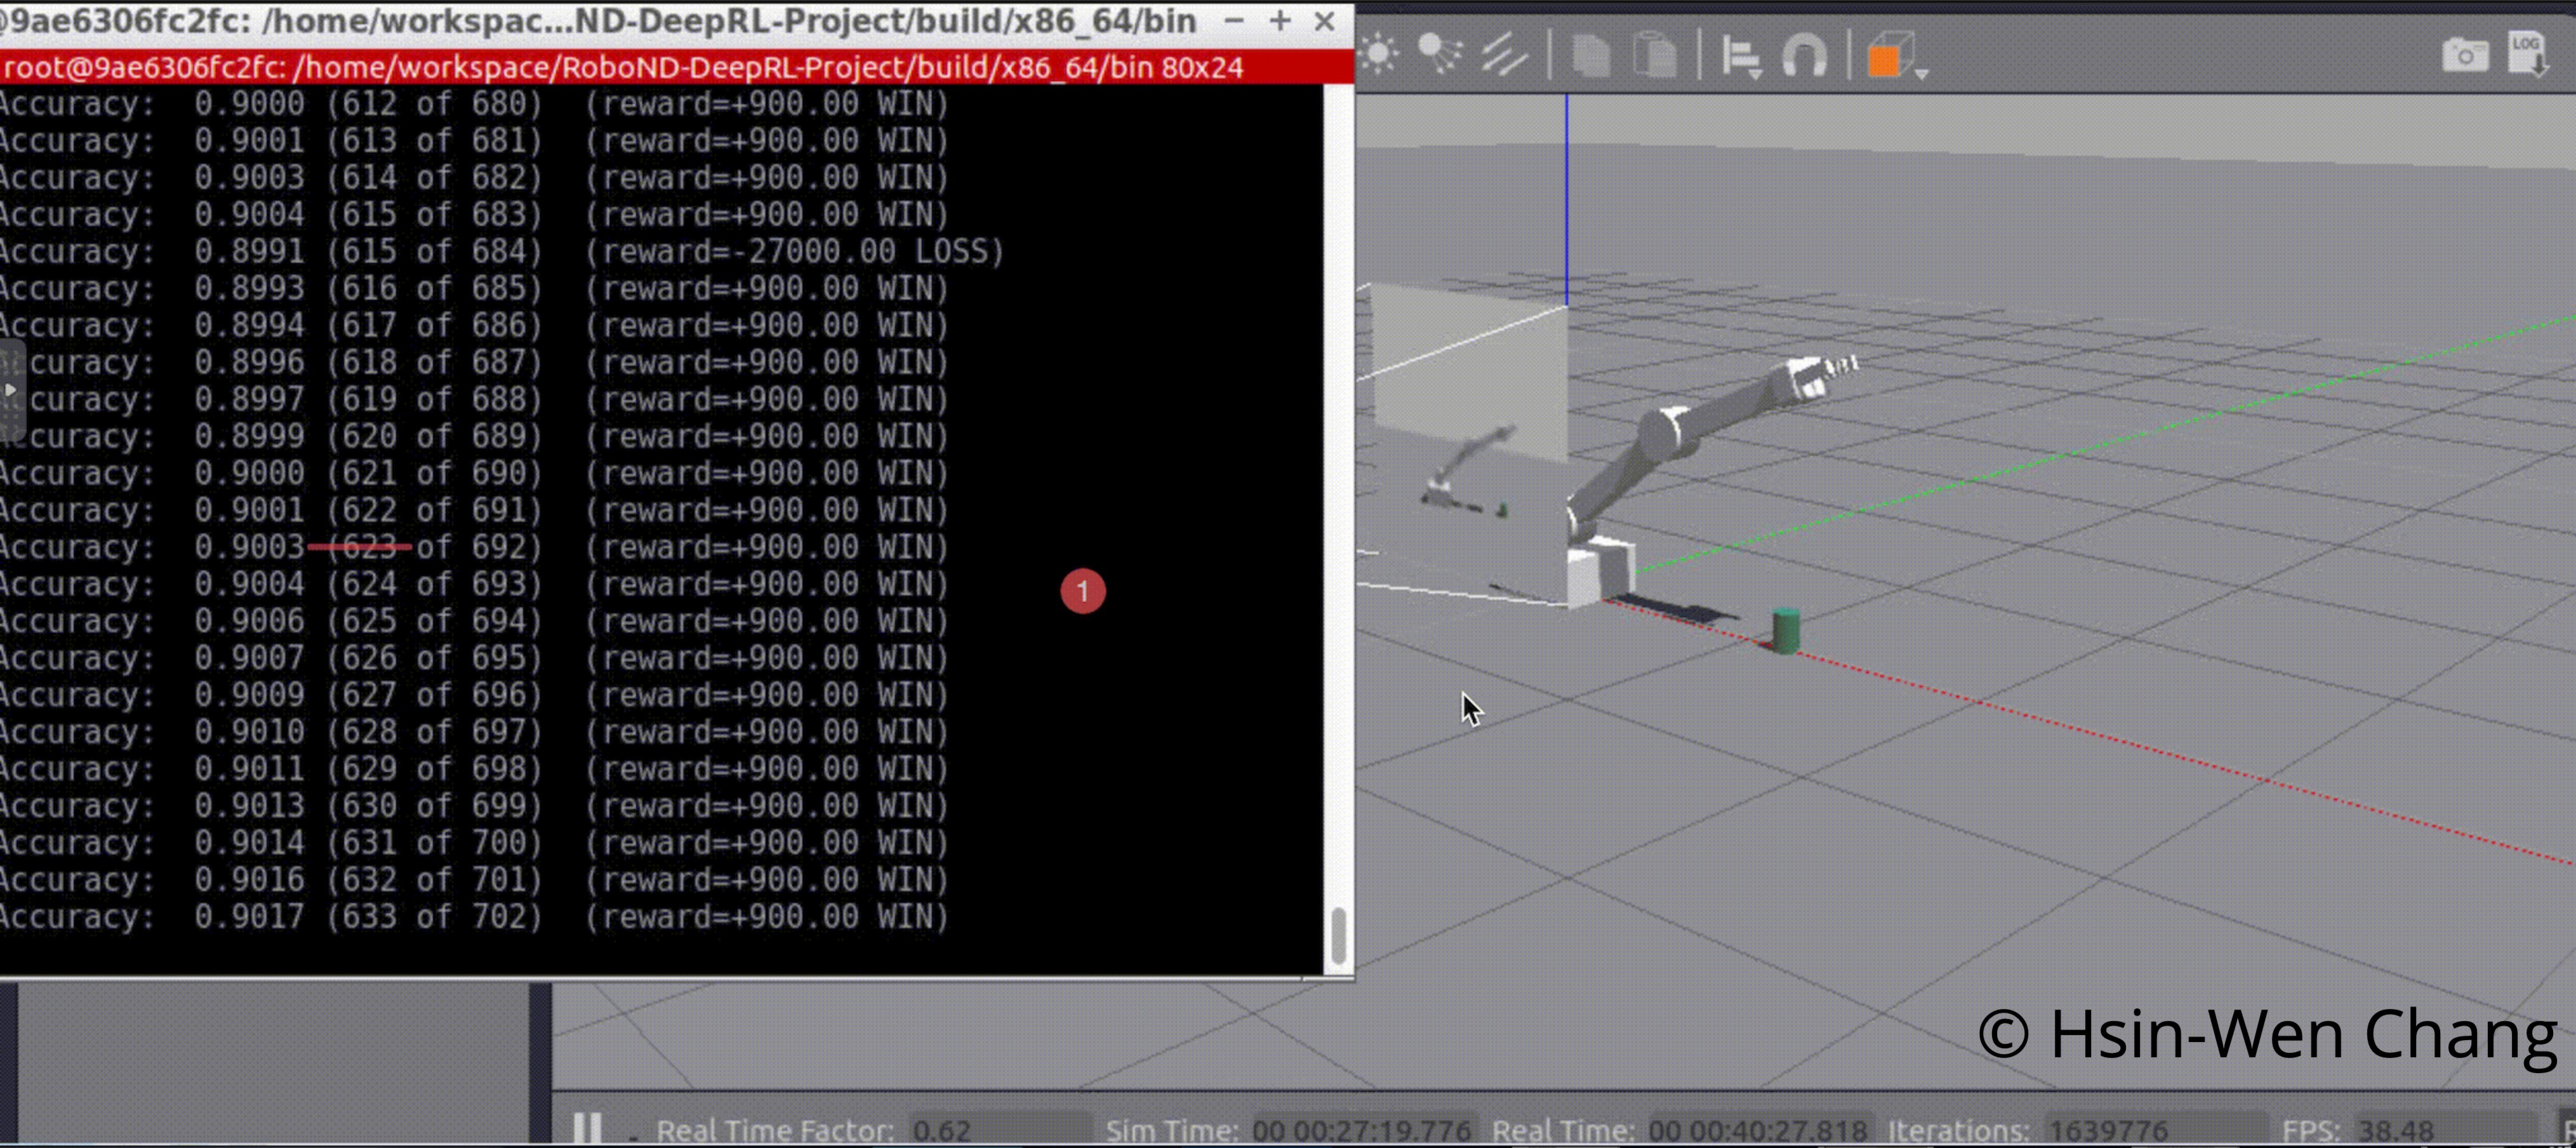
\includegraphics[width=\linewidth]{90.png}
      \caption{Achieved 90 percent.}
      \label{fig:achieved 90 percent}
\end{figure}
\item Have only the gripper base of the robot arm touch the object, with at least a 80 percent accuracy.
\begin{figure}[htpb]
      \centering
      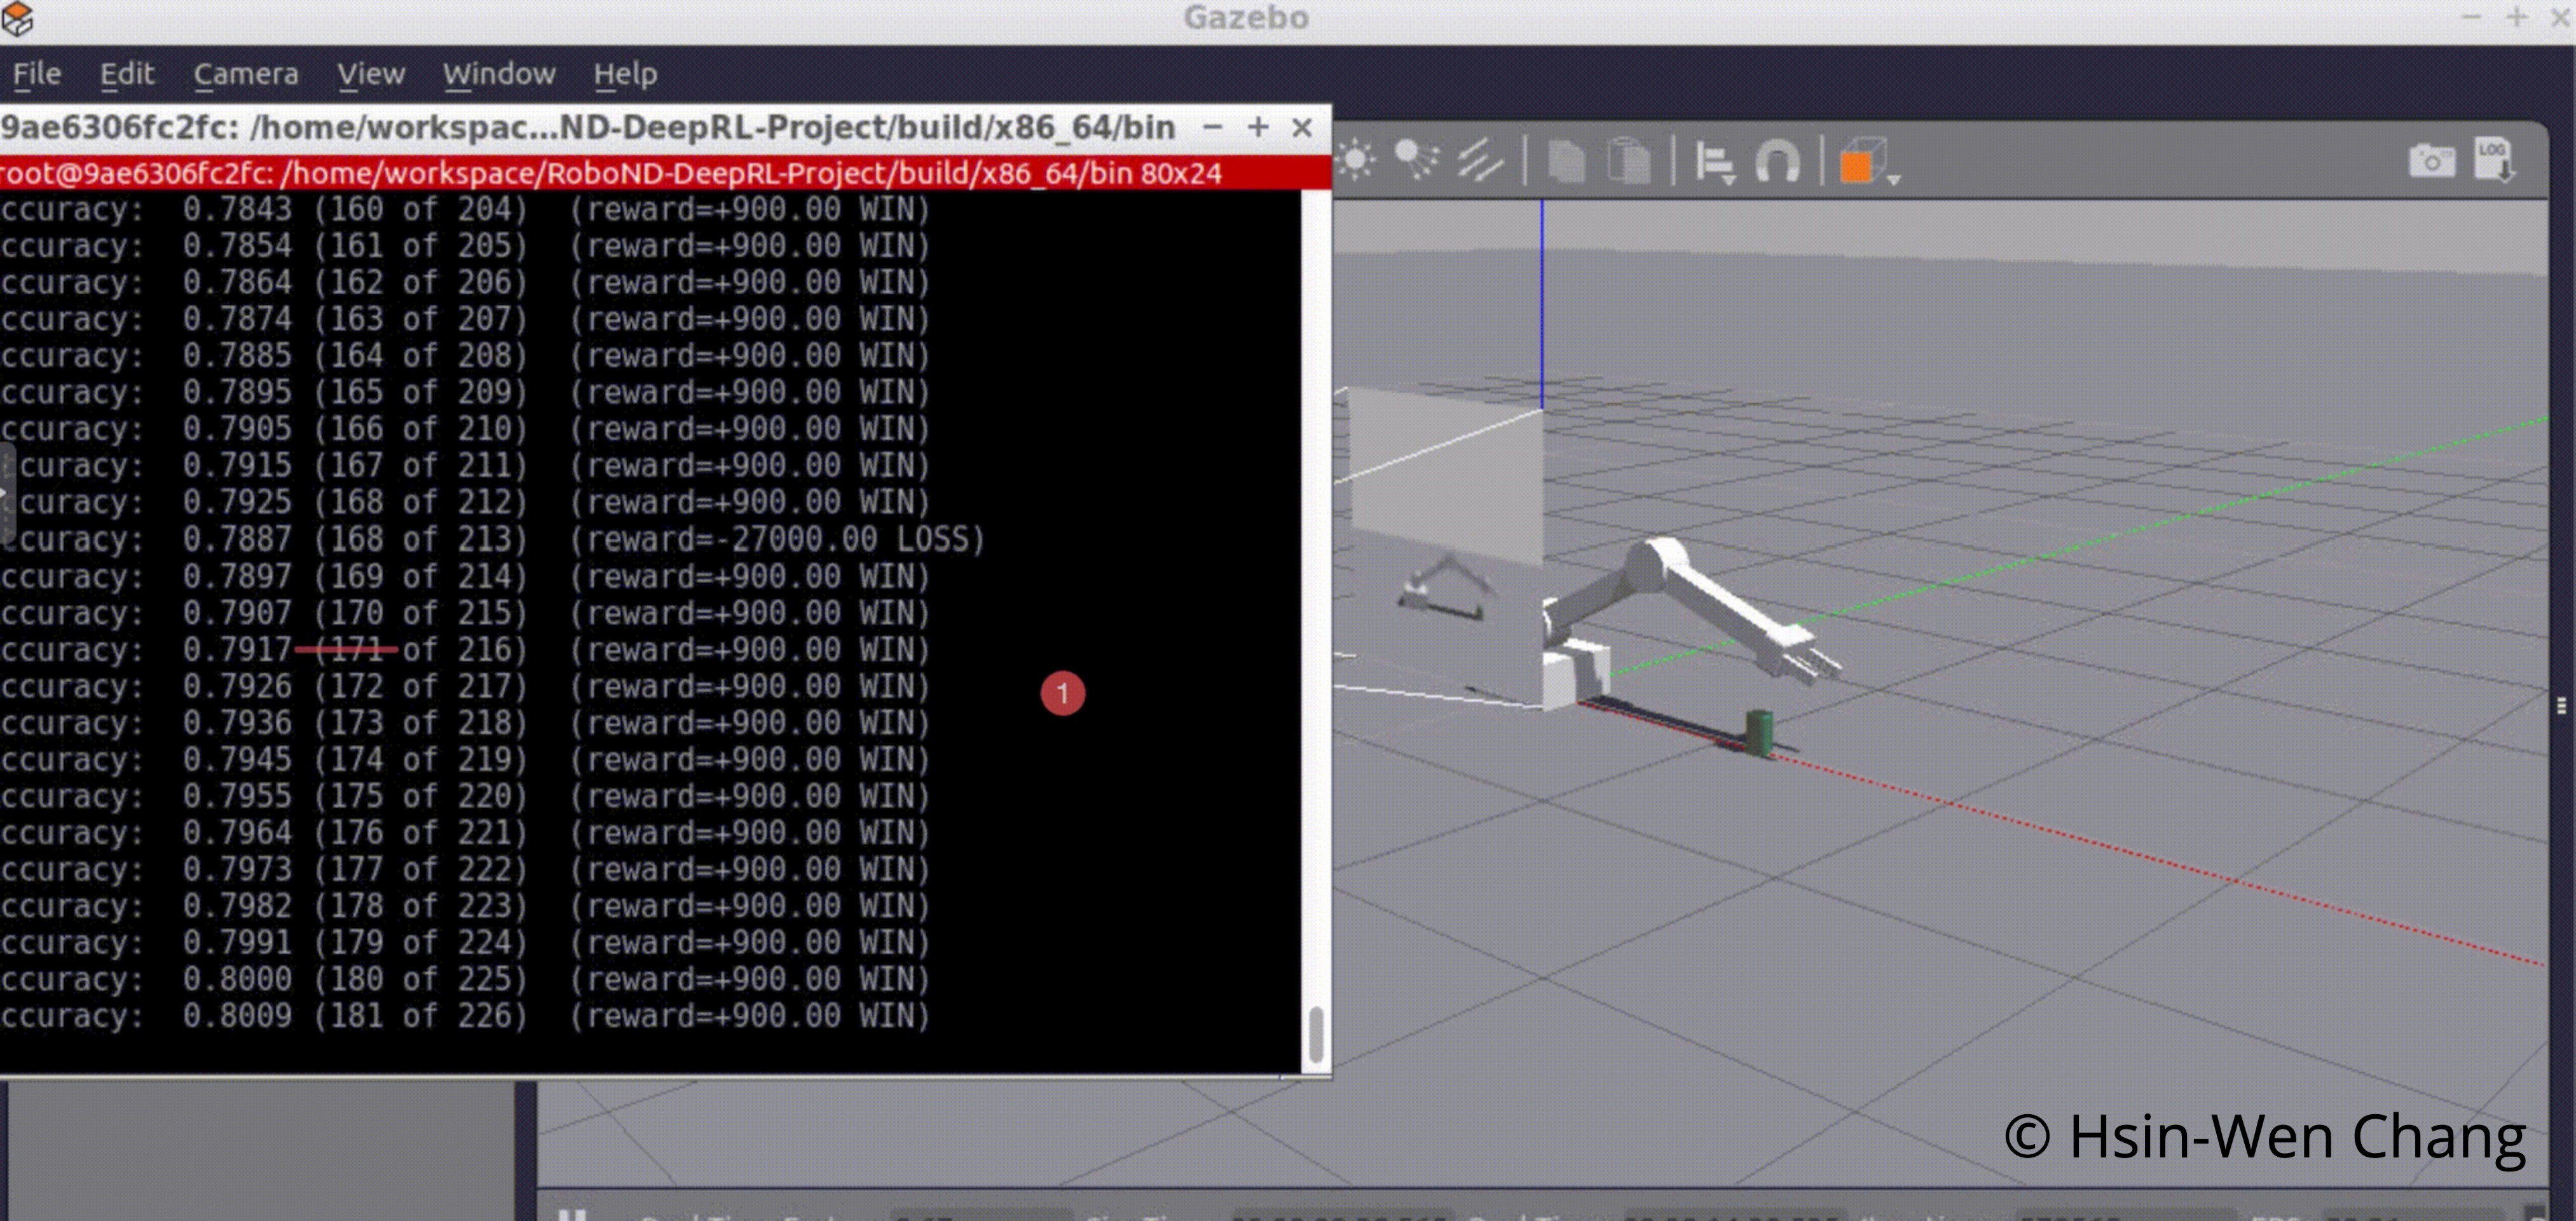
\includegraphics[width=\linewidth]{80.png}
      \caption{Achieved 80 percent}
      \label{fig:achieved 80 percent}
\end{figure}
\end {itemize}
As Observed if don't add time penalty the robotic arm will start trembly around it's target and if the LSTM size lower than 256 will take longer time to reach the target accuracy.

\section{Conclusion / Future work}
\end{document}
